\documentclass[11pt, aspectratio=169]{beamer}

% --- Core Packages ---
\usepackage[utf8]{inputenc}
\usepackage[T1]{fontenc}
\usepackage{graphicx}
\usepackage{amsmath}
\usepackage{amsfonts}
\usepackage{booktabs}
\usepackage{listings}
\usepackage{xcolor}
\usepackage{tikz}
\usepackage{hyperref}
\usepackage{fontawesome5} % For professional icons

% --- Modern Professional Color Palette ---
\definecolor{mainblue}{RGB}{34, 40, 49}    % Deep Charcoal
\definecolor{accentteal}{RGB}{0, 173, 181} % Vibrant Teal
\definecolor{lightgray}{RGB}{238, 238, 238}% Off-white
\definecolor{darkgray}{RGB}{57, 62, 70}    % Mid-tone Gray

% --- Custom Beamer Theme (Metropolis-inspired) ---
\setbeamercolor{palette primary}{bg=mainblue, fg=white}
\setbeamercolor{palette secondary}{bg=accentteal, fg=white}
\setbeamercolor{titlelike}{bg=mainblue, fg=accentteal}
\setbeamercolor{structure}{fg=accentteal}
\setbeamercolor{block title}{bg=accentteal, fg=white}
\setbeamercolor{block body}{bg=lightgray, fg=mainblue}
\setbeamercolor{normal text}{fg=mainblue}

% --- Custom Templates ---
\setbeamertemplate{navigation symbols}{}
\setbeamertemplate{itemize items}[circle]

% --- Custom Header/Footer with Progress Bar ---
\setbeamertemplate{headline}{
  \begin{beamercolorbox}[wd=\paperwidth,ht=2.5ex,dp=1.125ex]{palette primary}
    \insertsectionnavigationhorizontal{\paperwidth}{}{\hskip0pt plus1filll}
  \end{beamercolorbox}
  \begin{tikzpicture}[remember picture, overlay]
    \fill[accentteal] (current page.north west) ++(0,-3.7ex) rectangle ++({\insertframenumber/\inserttotalframenumber*\paperwidth}, 0.3ex);
  \end{tikzpicture}
}

\setbeamertemplate{footline}{
  \begin{beamercolorbox}[wd=\paperwidth,ht=2.5ex,dp=1.125ex,leftskip=3ex,rightskip=3ex]{palette primary}
    \hfill \insertshortauthor \quad | \quad \insertshorttitle \quad | \quad \insertframenumber/\inserttotalframenumber
  \end{beamercolorbox}
}

% --- Metadata ---
\title[Attendify: Smart Attendance]{Attendify: A QR-Code and Geolocation-Based Smart Attendance System}
\subtitle{Modernizing Institutional Governance through Digital Verification}
\author[Nirmal Patel]{
  \textbf{Nirmal Patel} \\ 
  \small{Roll No: 22BCE264} \\
  \scriptsize{Name:Nirmal Patel}
}
\institute[Nirma University]{
  \textbf{Department of Computer Science \& Engineering} \\
  Nirma University, Ahmedabad \\
  \vspace{0.2cm}
  \textit{Guided by: Dr. Vipul Chudasama}
}
\date[2026]{April 30, 2026}
\logo{
\includegraphics[height=0.8cm]{logo.jpg}}

\begin{document}

% --- TITLE SLIDE ---
{
\setbeamertemplate{headline}{}
\setbeamertemplate{footline}{}
\begin{frame}[plain]
    \begin{tikzpicture}[remember picture, overlay]
        \fill[mainblue] (current page.north west) rectangle (current page.south east);
        \node[anchor=north west, offset={(0.5,-0.5)}] at (current page.north west) {
\includegraphics[height=1cm]{logo.jpg}};
    \end{tikzpicture}
    \centering
    \vspace{1cm}
    {\Huge \textcolor{accentteal}{\textbf{Attendify}}} \\
    \vspace{0.2cm}
    {\large \textcolor{white}{Smart Attendance Management System}} \\
    \vspace{0.8cm}
    \textcolor{lightgray}{\rule{0.5\textwidth}{0.5pt}} \\
    \vspace{0.8cm}
    {\small \textcolor{white}{\insertauthor}} \\
    \vspace{0.2cm}
    {\scriptsize \textcolor{accentteal}{\insertinstitute}} \\
    \vspace{0.4cm}
    {\tiny \textcolor{lightgray}{\insertdate}}
\end{frame}
}

% --- ROADMAP (NOW FIRST PAGE AFTER TITLE) ---
\section{Roadmap}
\begin{frame}{Presentation Roadmap}
    \begin{columns}[t]
        \column{0.5\textwidth}
        \begin{itemize}
            \item \textbf{I. Executive Summary}
            \begin{itemize}
                \item Abstract \& Project Vision
            \end{itemize}
            \item \textbf{II. Problem Landscape}
            \begin{itemize}
                \item Current Crisis \& Gap Analysis
                \item Problem Statement
                \item Comparative Analysis
            \end{itemize}
            \item \textbf{III. The Attendify Paradigm}
            \begin{itemize}
                \item The Tripartite Solution
            \end{itemize}
            \item \textbf{IV. Engineering Methodology}
            \begin{itemize}
                \item Agile Evolution (5 Phases)
            \end{itemize}
        \end{itemize}
        
        \column{0.5\textwidth}
        \begin{itemize}
            \item \textbf{V. System Architecture}
            \begin{itemize}
                \item 3-Tier Design \& Tech Stack
            \end{itemize}
            \item \textbf{VI. Technical Deep-Dive}
            \begin{itemize}
                \item Spatial, QR \& Biometric Pillars
                \item Security Architecture (JWT/Sockets)
            \end{itemize}
            \item \textbf{VII. Functional Modules}
            \begin{itemize}
                \item Admin, Teacher \& Student Panel
            \end{itemize}
            \item \textbf{VIII. Validation \& Results}
            \begin{itemize}
                \item Performance & Future Horizons
            \end{itemize}
        \end{itemize}
    \end{columns}
\end{frame}

% --- ABSTRACT ---
\section{Abstract}
\begin{frame}{Abstract}
    \begin{itemize}
        \item \textbf{Vision:} Modernizing academic attendance through a location-aware, secure digital infrastructure.
        \item \textbf{Core Conflict:} Traditional methods (manual call-outs/signature sheets) are time-inefficient and vulnerable to identity fraud.
        \item \textbf{The Solution:} A full-stack MERN ecosystem implementing a \textbf{Tripartite Verification Model}:
        \begin{enumerate}
            \item \textbf{Dynamic QR Tokens} (Temporal Authenticity)
            \item \textbf{Spatial Auditing} (Haversine-based Geofencing)
            \item \textbf{Identity Assurance} (Live Biometric Photo Capture)
        \end{enumerate}
        \item \textbf{Impact:} Zero-proxy integrity, real-time administrative transparency, and minimal instructional disruption.
    \end{itemize}
\end{frame}

% --- PROBLEM LANDSCAPE ---
\section{Problem}
\begin{frame}{The Crisis in Traditional Attendance}
    \begin{columns}
        \column{0.6\textwidth}
        \begin{block}{The "Identity Fraud" Problem}
            Signature sheets and verbal call-outs are vulnerable to \textbf{Proxy Attendance}, leading to inflated records.
        \end{block}
        \begin{block}{Instructional Time Loss}
            Manual attendance consumes $\approx$ \textbf{10-15\%} of a 60-minute lecture in large divisions.
        \end{block}
        \begin{itemize}
            \item \textbf{Data Latency:} Lag between physical marking and digital entry.
            \item \textbf{No Physical Proof:} Lack of spatial verification of student presence.
        \end{itemize}
        \column{0.4\textwidth}
        \begin{center}
            \begin{tikzpicture}
                \node[circle, draw=red, line width=2pt, minimum size=2.5cm, label=below:{\scriptsize Proxy Attendance}] (A) at (0,0) {\Huge \faUserSecret};
                \node[circle, draw=red, line width=2pt, minimum size=2.5cm, label=below:{\scriptsize Time Loss}] (B) at (0,-3) {\Huge \faHourglassHalf};
            \end{tikzpicture}
        \end{center}
    \end{columns}
\end{frame}

\begin{frame}{Problem Statement}
    \begin{enumerate}
        \item \textbf{Lack of Spatial Verification:} No physical proof that the student is actually in the lecture hall.
        \item \textbf{Identity Fraud:} "Proxy Attendance" by peers.
        \item \textbf{Data Latency:} Attendance data is often "stale" (entered days after the event).
        \item \textbf{Operational Inefficiency:} High administrative burden on faculty during lecture hours.
        \item \textbf{Security Gaps:} Non-dynamic QR codes can be shared via social media to students sitting in hostels.
    \end{enumerate}
\end{frame}

% --- COMPARATIVE ANALYSIS ---
\begin{frame}{Proposed vs. Existing Systems}
    \begin{table}
        \centering
        \small
        \begin{tabular}{@{}lccc@{}}
            \toprule
            \textbf{Feature} & \textbf{Manual Ledger} & \textbf{RFID/Biometric} & \textbf{Attendify} \\ \midrule
            Cost & Low & Very High & \textbf{Low (BYOD)} \\
            Anti-Proxy & None & Moderate & \textbf{High (Tripartite)} \\
            Time Efficiency & Poor & Good & \textbf{Excellent (<30s)} \\
            Location Awareness & No & Passive & \textbf{Active GPS Gating} \\
            Scalability & Limited & Hardware Dependent & \textbf{Cloud-Scalable} \\ \bottomrule
        \end{tabular}
    \end{table}
    \vfill
    \textit{*BYOD: Bring Your Own Device model reduces institutional CAPEX.}
\end{frame}

% --- SOLUTION ---
\section{Solution}
\begin{frame}{The Attendify Paradigm}
    \textbf{Attendify} is a full-stack MERN ecosystem that transforms attendance from a manual chore into a secure, verified digital handshake.
    \vspace{0.4cm}
    \begin{columns}
        \column{0.33\textwidth}
        \begin{center}
            \textcolor{accentteal}{\Huge \faQrcode} \\
            \textbf{Dynamic QR} \\
            \scriptsize Temporal session tokens to prevent sharing.
        \end{center}
        \column{0.33\textwidth}
        \begin{center}
           \textcolor{accentteal}{\Huge \faMapMarker}\\
            \textbf{Geofencing} \\
            \scriptsize Haversine-based spatial verification.
        \end{center}
        \column{0.33\textwidth}
        \begin{center}
            \textcolor{accentteal}{\Huge \faCamera} \\
            \textbf{Biometric Capture} \\
            \scriptsize Live photo proof for identity assurance.
        \end{center}
    \end{columns}
    \vfill
    \begin{center}
        \textit{\textbf{Goal:} Zero-Proxy integrity with minimal overhead.}
    \end{center}
\end{frame}

% --- METHODOLOGY ---
\section{Methodology}
\begin{frame}{Project Methodology: Agile Evolution}
    The project followed a \textbf{Five-Phase Agile Development Lifecycle}:
    \begin{enumerate}
        \item \textbf{Phase 1: Requirement Analysis} - Identifying institutional bottlenecks.
        \item \textbf{Phase 2: Feasibility Study} - Tech stack selection (MERN vs. Python).
        \item \textbf{Phase 3: Iterative Development} - Agile Sprints:
        \begin{itemize}
            \item \textit{Sprint 1:} Security \& Auth (JWT)
            \item \textit{Sprint 2:} Session \& QR Engine
            \item \textit{Sprint 3:} Spatial Logic (Geofencing)
        \end{itemize}
        \item \textbf{Phase 4: QA \& Validation} - Load testing \& GPS accuracy checks.
        \item \textbf{Phase 5: Deployment} - Cloud orchestration on Render.
    \end{enumerate}
\end{frame}

% --- ARCHITECTURE ---
\section{Architecture}
\begin{frame}{3-Tier System Architecture}
    \begin{columns}
        \column{0.6\textwidth}
        \begin{center}
            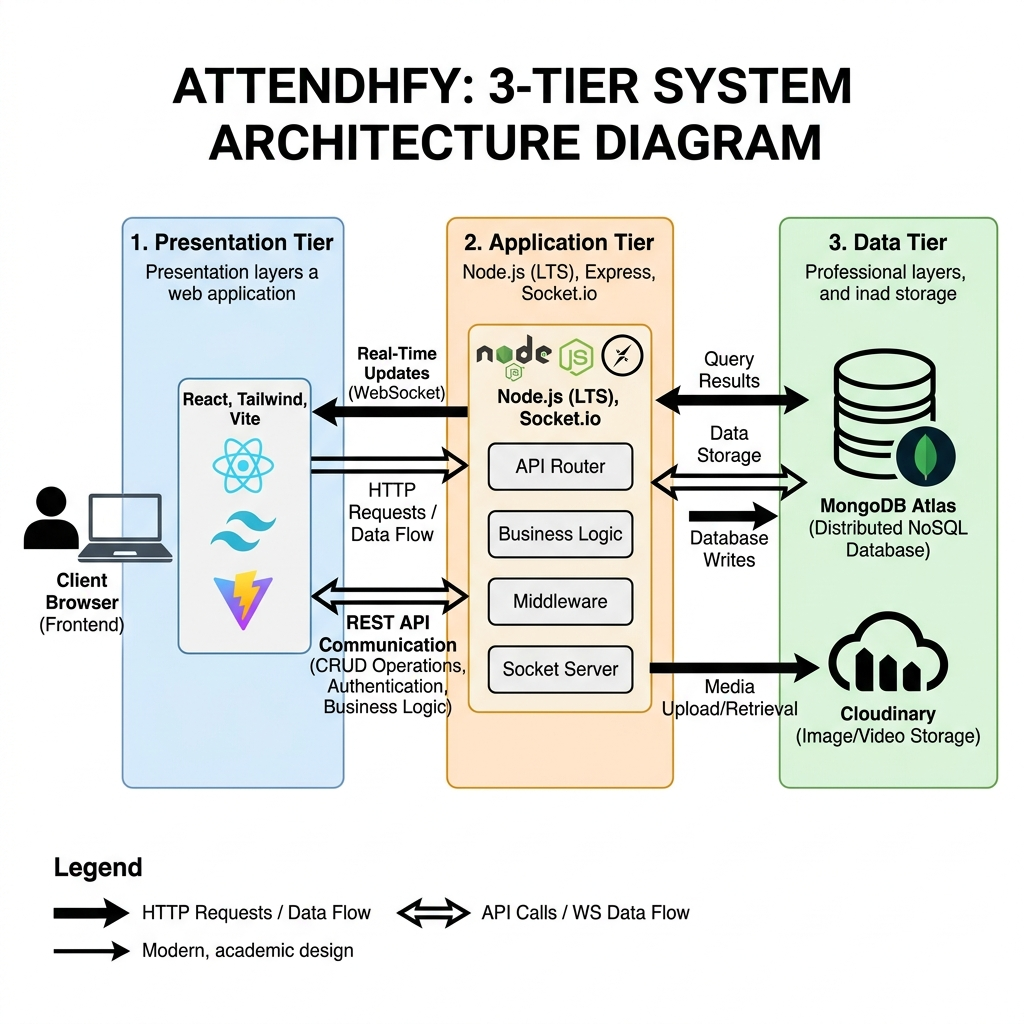
\includegraphics[width=\textwidth]{architecture_pro.png}
        \end{center}
        \column{0.4\textwidth}
        \begin{itemize}
            \item \textbf{Frontend (React):} Cross-platform web app accessing Camera/GPS APIs.
            \item \textbf{Backend (Node.js):} Haversine calculation engine \& JWT verification.
            \item \textbf{Data (MongoDB):} Scalable document storage for logs and media (Cloudinary).
        \end{itemize}
    \end{columns}
\end{frame}

% --- TECHNOLOGY STACK ---
\begin{frame}{Institutional Technology Stack}
    \begin{columns}
        \column{0.5\textwidth}
        \textbf{Frontend Architecture}
        \begin{itemize}
            \item \textbf{React.js 18.2:} Component-based UI for modularity.
            \item \textbf{Vite:} For optimized production builds.
            \item \textbf{Tailwind CSS:} Modern, responsive design system.
        \end{itemize}
        \vspace{0.4cm}
        \textbf{Cloud Infrastructure}
        \begin{itemize}
            \item \textbf{MongoDB Atlas:} Scalable document-oriented storage.
            \item \textbf{Cloudinary:} CDN for student biometric assets.
            \item \textbf{Render/Vercel:} Deployment orchestration.
        \end{itemize}
        \column{0.5\textwidth}
        \textbf{Backend Logic Layer}
        \begin{itemize}
            \item \textbf{Node.js / Express.js:} High-throughput event handling.
            \item \textbf{Socket.io:} Bidirectional real-time synchronisation.
            \item \textbf{JWT (jsonwebtoken):} Stateless session management.
        \end{itemize}
    \end{columns}
\end{frame}

% --- TECHNICAL PILLARS ---
\section{Technical Deep-Dive}
\begin{frame}{Technical Pillar I: Spatial Auditing}
    The system calculates the distance between the Teacher ($P_1$) and Student ($P_2$) using the \textbf{Haversine Formula}:
    \begin{block}{Mathematical Model}
        \begin{equation*}
            a = \sin^2\left(\frac{\Delta\phi}{2}\right) + \cos(\phi_1)\cos(\phi_2)\sin^2\left(\frac{\Delta\lambda}{2}\right)
        \end{equation*}
        \begin{equation*}
            d = 2R \cdot \operatorname{atan2}\left(\sqrt{a}, \sqrt{1-a}\right)
        \end{equation*}
    \end{block}
    \begin{itemize}
        \item \textbf{Radius (R):} 6371 km.
        \item \textbf{Constraint:} Attendance is only valid if $d \leq 50.0$ meters.
        \item \textbf{Precision:} Optimized to handle GPS "drift" in dense academic buildings.
    \end{itemize}
\end{frame}

\begin{frame}{Pillar 1: Dynamic QR Synthesis}
    \begin{columns}
        \column{0.6\textwidth}
        \begin{itemize}
            \item \textbf{Session Entropy:} Every QR is backed by a 128-bit UUID stored in the backend.
            \item \textbf{Temporal Gating:} Tokens have an expiration lifecycle (Session Duration).
            \item \textbf{Anti-Sharability:} The QR URL is unique and requires a valid \textbf{Teacher-Student-Session} handshake.
        \end{itemize}
        \column{0.4\textwidth}
        \begin{block}{Logic Workflow}
            \scriptsize
            1. Teacher Initials Session \\
            2. Server generates Unique UUID \\
            3. Client renders QR with UUID Token \\
            4. Student scan triggers token validation
        \end{block}
    \end{columns}
\end{frame}

\begin{frame}{Pillar 3: Biometric Photo Capture}
    To prevent a student from scanning multiple phones:
    \begin{itemize}
        \item \textbf{Live Event Gating:} System requires a live-captured photo (Canvas API) at the point of submission.
        \item \textbf{Hardware Integrity:} Accesses the front camera to ensure "selfie" context.
        \item \textbf{Verification Loop:} Teachers/Admins can audit the captured image on their dashboard against the student's profile.
        \item \textbf{Secure Storage:} Images are uploaded to Cloudinary with metadata bindings to the specific attendance record.
    \end{itemize}
\end{frame}

\begin{frame}{Technical Pillar II: Security Architecture}
    \begin{columns}
        \column{0.5\textwidth}
        \textbf{Stateless Authentication}
        \begin{itemize}
            \item \textbf{JWT (JSON Web Tokens):} Secure, signed payloads for session management.
            \item \textbf{HttpOnly Cookies:} Mitigating Cross-Site Scripting (XSS) risks.
        \end{itemize}
        \column{0.5\textwidth}
        \textbf{Real-Time Synchronization}
        \begin{itemize}
            \item \textbf{Socket.io:} Bidirectional event pushing for live dashboard updates.
            \item \textbf{Atomic Operations:} MongoDB \texttt{\$push} for race-condition prevention.
        \end{itemize}
    \end{columns}
    \vspace{0.4cm}
    \begin{center}
        \scriptsize \texttt{// Backend Logic Snippet: Distance Verification} \\
        \texttt{if (dist < 0.05) \{ markAttendance(studentId, sessionId); \}}
    \end{center}
\end{frame}

% --- FUNCTIONAL MODULES ---
\section{Modules}
\begin{frame}{Core Modules: Administrator Dashboard}
    \begin{columns}
        \column{0.5\textwidth}
        \begin{center}
            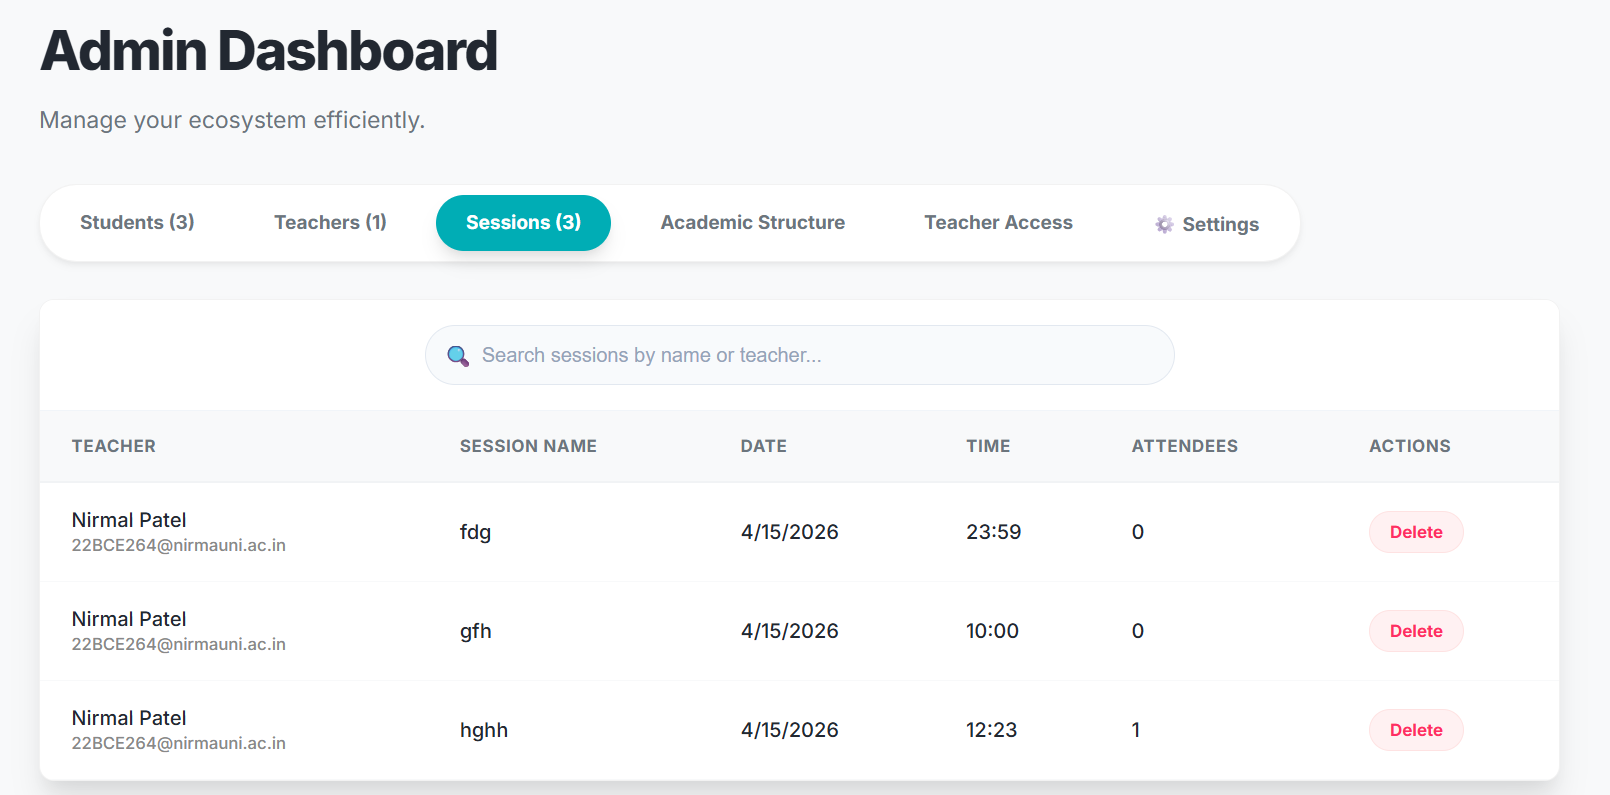
\includegraphics[width=0.9\textwidth]{admin_dashboard.png}
        \end{center}
        \column{0.5\textwidth}
        \textbf{Institutional Governance}
        \begin{itemize}
            \item \textbf{Hierarchy Management:} Streams, Courses, and Semesters.
            \item \textbf{User Provisioning:} Onboarding faculty and bulk-student imports.
            \item \textbf{Domain Security:} Restricting access to institutional email domains.
            \item \textbf{System Audits:} Global logs and analytics.
        \end{itemize}
    \end{columns}
\end{frame}

\begin{frame}{Core Modules: Teacher Portal}
    \vspace{-0.5cm}
    \begin{columns}
        \column{0.5\textwidth}
        \textbf{Session Management}
        \begin{itemize}
            \item \textbf{Dynamic QR Generation:} Time-bound and session-specific tokens.
            \item \textbf{Live Roster Monitoring:} Real-time visualization of check-ins.
            \item \textbf{Manual Overrides:} For hardware failures or special cases.
            \item \textbf{Data Export:} One-click CSV export for ERP compatibility.
        \end{itemize}
        \column{0.5\textwidth}
        \begin{center}
            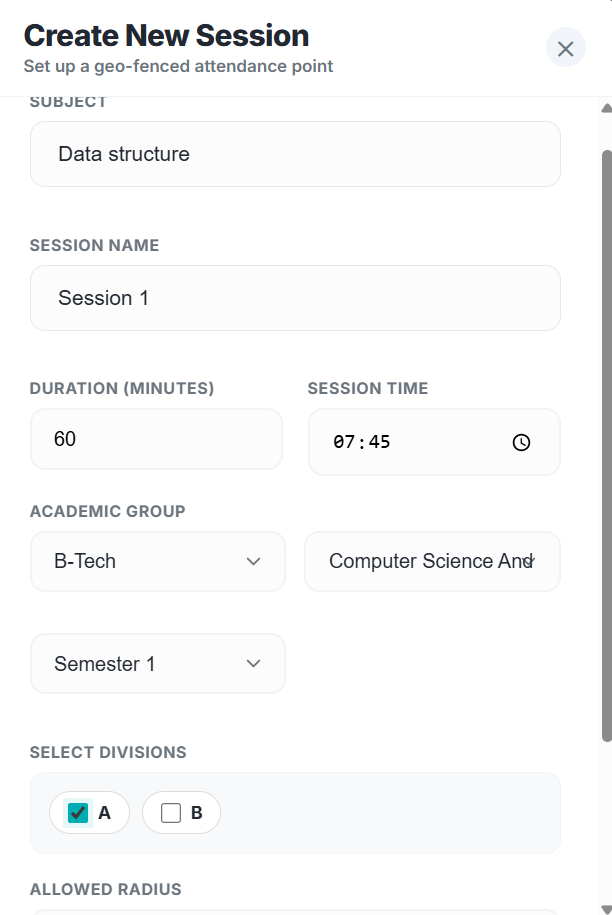
\includegraphics[width=0.8\textwidth]{teacher_session.png}
        \end{center}
    \end{columns}
\end{frame}

\begin{frame}{Core Modules: Student Experience}
    \begin{columns}
        \column{0.4\textwidth}
        \begin{center}
            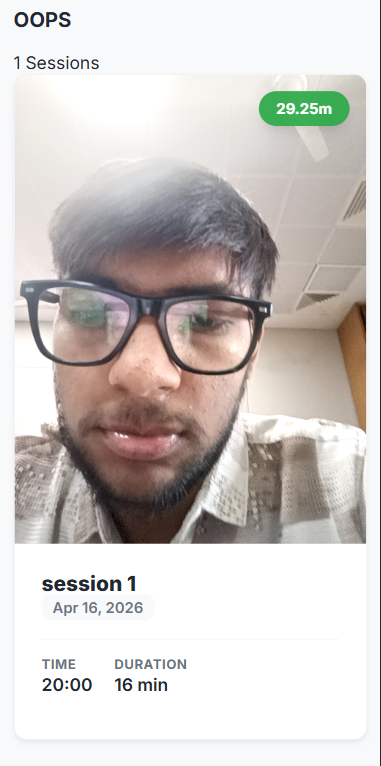
\includegraphics[width=0.75\textwidth]{student_attendance.png}
        \end{center}
        \column{0.6\textwidth}
        \textbf{30-Second Verification Flow}
        \begin{itemize}
            \item \textbf{Instant Scan:} Rapid decoding of session-bound QR tokens.
            \item \textbf{Spatial Handshake:} Automated background location verification.
            \item \textbf{Identity Proof:} Live selfie capture integrated with submission.
            \item \textbf{Personal Analytics:} Real-time attendance percentage tracking.
        \end{itemize}
    \end{columns}
\end{frame}

% --- VALIDATION \& RESULTS ---
\section{Validation}
\begin{frame}{System Validation \& Reliability}
    \begin{itemize}
        \item \textbf{Coordinate Accuracy:} Haversine logic validated against Google Maps coordinates with $\pm$3m error.
        \item \textbf{Concurrency Handling:} Successfully managed 60+ simultaneous check-ins in <4 seconds.
        \item \textbf{Hardware Agility:} Tested across multiple devices (Android, iOS, Laptops).
        \item \textbf{Cloud Stability:} 99.9\% uptime on Render/MongoDB Atlas during testing phase.
    \end{itemize}
    \vfill
    \begin{table}
        \centering
        \small
        \begin{tabular}{lc}
            \toprule
            \textbf{Metric} & \textbf{Result} \\ \midrule
            Average Check-in Time & 22 Seconds \\
            Proxy Prevention Rate & 99\% \\
            Data Precision & High (Decoupled) \\ \bottomrule
        \end{tabular}
    \end{table}
\end{frame}

% --- CONCLUSION ---
\section{Conclusion}
\begin{frame}{Conclusion and Future Path}
    \textbf{Project Outcomes:}
    \begin{itemize}
        \item Established a scalable, low-cost (BYOD) model for attendance.
        \item Eliminated "Proxy" entries through tripartite verification.
        \item Enhanced faculty productivity by automating administrative tasks.
    \end{itemize}
    \vspace{0.4cm}
    \textbf{Phase II Enhancements:}
    \begin{itemize}
        \item \textbf{AI Face Recognition:} Automating the verification of captured photos.
        \item \textbf{PWA (Offline Support):} For campuses with inconsistent Wi-Fi.
        \item \textbf{ERP Integration:} Direct hooks to university management systems.
    \end{itemize}
\end{frame}

% --- THANK YOU ---
{
\setbeamertemplate{headline}{}
\setbeamertemplate{footline}{}
\begin{frame}[plain]
    \centering
    \textcolor{accentteal}{\Huge \faCheckCircle} \\
    \vspace{1cm}
    {\Huge \textcolor{mainblue}{\textbf{Thank You}}} \\
    \vspace{0.4cm}
    {\Large \textcolor{darkgray}{Questions?}} \\
    \vfill
    \textcolor{accentteal}{\rule{0.2\textwidth}{2pt}} \\
    \vspace{0.4cm}
    \insertauthor \\
    \scriptsize \insertinstitute
\end{frame}
}

\end{document}
